\chapter{LES and SGS model}\label{LES}
\section{The concept of LES}
The idea behind large eddy simulations (LES) is to solve the filtered equations
of fluid dynamics (FE) \eqref{eq:filmsum} - \eqref{eq:etsum} instead of the
unfiltered ones (UE) \eqref{eq:mass}-\eqref{eq:etot}. There are two reasons for
this:
\begin{enumerate}
\item The FE represent a system with a smaller
number of resolved degrees of freedom (DOF) compared with the UE. This is a
necessary restriction, because the numerical discretization itself acts as a
filter\footnote{See section \ref{expfil}.} and limits the number of DOF which we
can resolve in a high Reynolds number flow. In effect this leads to the problem
that the outcome of a simulation of turbulence using the UE depends on the
numerical scheme used. If instead we solve the FE using a certain subgrid model
with a characteristic cutoff length higher than the numerical cutoff length, the
outcome of the turbulence simulation is only dependent on our subgrid model and
not on the numerical scheme used \citep{Mason1999}. From this point of view, we
should call a turbulence model simply a filter model.
\item Using the numerical cutoff as an explicit filter in an energy
conserving numerical scheme converts kinetic into internal energy. But
the back reaction of the internal energy on the kinetic energy can only be 
via the pressure term, which is presumably not right. With an explicit
turbulence model, we can model the backscattering of small scale fluctuations
on the resolved kinetic energy in a much better way \citep{Schmidt2004}. To
model the backscattering we have to know explicitly the amount of energy on the
scales between the cutoff scale and the Kolmogorov scale. This is what we call
subgrid energy or turbulent energy and that is why the term subgrid scale 
(SGS) model is appropriate for the unknown terms in the FE.
\end{enumerate}

Unfortunately there is a substantial variety of SGS models in the literature
and no agreement on a standard model. An extensive overview of SGS models for
incompressible flows can be found for example in the book by \citet{Sagaut2006}.
There are fewer models explicitly for compressible flows. A simple one,
that was first introduced by \citet{Schmidt2004,Schmidt2006a}, will
be described in the next sections. This \emph{Schmidt model}\footnote{Actually
the original implementation of the SGS model proposed by \citet{Schmidt2006a}
had severe problems with energy conservation and was notoriously difficult to
implement in an AMR code. The version of the \emph{Schmidt model} described in
this work is a simplified version, but it conserves energy and proved to be
sufficient for our work.}, together with some
corrections due to \citet{Sarkar1992}, which will be outlined later, is the
model we use to describe the influence of turbulence on the resolved scales
in our work.

\section{Schmidt model} 
As we interpret the trace of the generalized central moment of the
velocity $\fil{\tau}_{ij}$ as a turbulent energy, we can define a
velocity of the turbulent motions\footnote{This is 
based on an analogy to kinetic energy in the sense, that 
$\frac{1}{2}\rho q^2 = \rho e_t$.} $q=\sqrt{2 e_t}$, which is used as
characteristic velocity of the subgrid terms in the Schmidt model. As a
characteristic length scale the size of one grid cell $l_{\Delta}$ is used
\footnote{As mentioned, the implicit cutoff of our subgrid = filter model
should be greater than the numerical cutoff, so one might object, that 
$l_{\Delta}$ is too small for that. But every term in the subgrid model is
multiplied by some dimensionless constant, which is set to a value high enough
to make numerical cutoff effects insignificant.}.

The Schmidt model neglects the convective flux term
$\hat{\tau}(v_j,e_{int})$ and the gravitational effects $\Gamma$ on the subgrid
scales. The models for the other terms are described in the following sections.

\subsection{Transport term \texorpdfstring{$\mathbb{D}$}{D}}
The transport or diffusion term is modeled by a gradient hypothesis, by stating
that the non-linear term is proportional to the turbulent velocity $q^2$
gradient (Kolmogorov-Prandl relation, see \citet[p.97]{Sagaut2006})
\begin{align}
\mathbb{D}=\pd{r_i}C_{\mathbb{D}}\fil{\rho} l_{\Delta} q^2 \pd{r_i} q.
\end{align}
The constant $C_{\mathbb{D}}$ is
calibrated to $C_{\mathbb{D}} \approx 0.4 = \frac{2}{5}$ by
numerical experiments \citep{Schmidt2006}.

\subsection{Pressure dilatation \texorpdfstring{$\lambda$}{lambda}}
For $\lambda$ an estimate is used that is presumably only valid in the
subsonic (nearly incompressible) regime:
\begin{align}
\lambda=C_{\lambda} q^2 \pd{r_i}\hat{v}_i.
\end{align}
The constant $C_{\lambda}=-\frac{1}{5}$ as found by numerical experiments
\citep{Schmidt2006}.

\subsection{Turbulent dissipation
\texorpdfstring{$\epsilon$}{epsilon}}
The turbulent dissipation accounts for effects of viscosity on subgrid scales.
These effects convert turbulent energy to internal energy even if, on the
larger scales, the effect of viscosity can be neglected. The most simple
expression which can be built from the characteristic turbulent velocity and
length scale for the dissipation is
\begin{align}
\epsilon=C_{\epsilon}\frac{q^3}{l_{\Delta}}. \label{eq:epsmodel}
\end{align}
For our simulations we will set $C_{\epsilon}=0.5$.\footnote{Suggested by
W. Schmidt, personal communication.}

\subsection{Turbulence production tensor
\texorpdfstring{$\hat{\tau}(v_i,v_j)$}{tau}}
The turbulence production term is symmetric in its arguments and can
therefore be written as follows
\begin{align}
\hat{\tau}(v_i,v_j)=\hat{\tau}_{ij}=\frac{1}{2}(\hat{\tau}_{ij}+\hat{\tau}_{ij}
)
=\frac{1}{2}(\hat{\tau}_{ij}+\hat{\tau}_{ji}).
\end{align}
By subtracting the trace of this tensor
\begin{align}
\hat{\tau}_{ij}=\frac{1}{2}(\hat{\tau}_{ij}+\hat{\tau}_{ji})
-\frac{1}{n}\delta_{ij}\hat{\tau}_{kk}+\frac{1}{3}\delta_{ij}\hat{\tau}_{kk}
\end{align}
and recognizing that $\hat{\tau}_{kk}=\fil{\rho} q^2 $ we can split the tensor
in a symmetric, tracefree part 
$\hat{\tau}^*_{ij}=\frac{1}{2}(\hat{\tau}_{ij}+\hat{\tau}_{ji})
-\frac{1}{3}\delta_{ij}\hat{\tau}_{kk}$ and the trace
\begin{align}
\hat{\tau}_{ij}=\hat{\tau}^*_{ij}+\frac{1}{3}\delta_{ij}\fil{\rho}q^2 =
\hat{\tau}^*_{ij} + p_t,
\end{align}
where the trace is commonly called turbulent pressure $p_t$.

A model for $\hat{\tau}^*_{ij}$ is based on the turbulent viscosity
hypothesis.
There it is assumed, that $\hat{\tau}^*_{ij}$ is of the same form like
$S^*_{ij}$ for a newtonian fluid, so
\begin{align}
\hat{\tau}^*_{ij}=- 2 \eta_t S^*_{ij}
\end{align}
with a turbulent dynamic viscosity
$\eta_t=\fil{\rho}\nu_t=\fil{\rho}C_{\nu}l_{\Delta} q$ and
\begin{align}
S^*_{ij}=\frac{1}{2}\lra{\pd{r_j}\hat{v}_i+\pd{r_i}\hat{v}_j}
-\frac{1}{3}\delta_{ij}\pd{r_k}\hat{v}.
\end{align}
The turbulence production term is therefore modeled as
\begin{align}
\hat{\tau}(v_i,v_j)=-2\fil{\rho}C_{\nu} l_{\Delta} q
S^*_{ij}+\frac{1}{3}\delta_{ij}\fil{\rho}q^2.
\end{align}

It should be noted, that in general the old idea of turbulent viscosity
(which was first forumlated by \citet{Boussinesq1877}) is
incorrect. As \citet{Pope2000} shows, it
is only true when the ratio of production of turbulent energy
$\Sigma^*=\hat{\tau}^*_{ij}\ppd{r_j}{v_i}$ to dissipation $\epsilon$ is
$\frac{\Sigma^*}{\epsilon}\sim 1$. If this ratio is much greater or much
smaller than one the turbulent viscosity hypothesis is incorrect. 

Nevertheless since it is the most common idea used to model the turbulent
production tensor it is also used in the Schmidt model. Setting the
constant $C_{\nu}=0.05$ seems to be a rational choice \citep{Schmidt2006}.

\subsection{Summary of the Schmidt model}
Using the Schmidt model, the FE form the following system of equations
\begin{align}
\pd{t}\fil{\rho} + \pd{r_j}\hat{v}_j\fil{\rho} =&\ 0,\\
\pd{t}\fil{\rho}\hat{v}_i + \pd{r_j}\hat{v}_j\fil{\rho}\hat{v}_i =&
-\pd{r_i}(\fil{p}+p_t)+\fil{\rho}\hat{g}_i
-\pd{r_j}\hat{\tau}^*_{ij},
\\
\begin{split}
\pd{t}\fil{\rho}e_{res}+\pd{r_j}\hat{v}_j\fil{\rho}e_{res}=&
-\pd{r_i}\hat{v}_i(\fil{p}+p_t)
+\fil{\rho}\hat{v}_i\hat{g}_i\\
&+\fil{\rho}(\lambda+\epsilon)
-\hat{v}_i\pd{r_j}\hat{\tau}^*(v_i,v_j),
)
\end{split}
\\
\pd{t}\fil{\rho}e_t+\pd{r_j}\hat{v}_j
\fil{\rho}e_t=&\ \mathbb{D}-\fil{\rho}(\lambda+\epsilon)
-\hat{\tau}^*(v_j,v_i)\pd{r_j}\hat{v_i}-p_t\pd{r_i}\hat{v_i}.
\end{align}
Again it is often useful to split the equation for resolved energy into an
equation for the resolved kinetic energy and internal energy respectively
\begin{align}
\begin{split}
\pd{t}\fil{\rho} \hat{e}_k+\pd{r_j}\hat{v}_j \fil{\rho} \hat{e}_k) =& 
-\hat{v}_i \pd{r_i}(\fil{p}+p_t)
+\fil{\rho} \hat{v}_i \hat{g}_i
-\hat{v}_i\pd{r_j}\hat{\tau}^*(v_i,v_j),
\end{split}
\\
\begin{split}
\pd{t}\fil{\rho} \hat{e}_{int}+\pd{r_j}\hat{v}_j \fil{\rho} \hat{e}_{int} =&
-(\fil{p}+p_t) \pd{r_j}\hat{v}_j
+\fil{\rho}(\lambda+\epsilon).
\end{split}
\end{align}

\section{Impact of the Schmidt SGS on the fluid equations}\label{ImpactSGS}
\subsection{General observations}
In this section we want to investigate the influence of the Schmidt model on
the equations of fluid dynamics. This can be done most easily in a graphical
way.

\begin{figure}[tp]
\centering
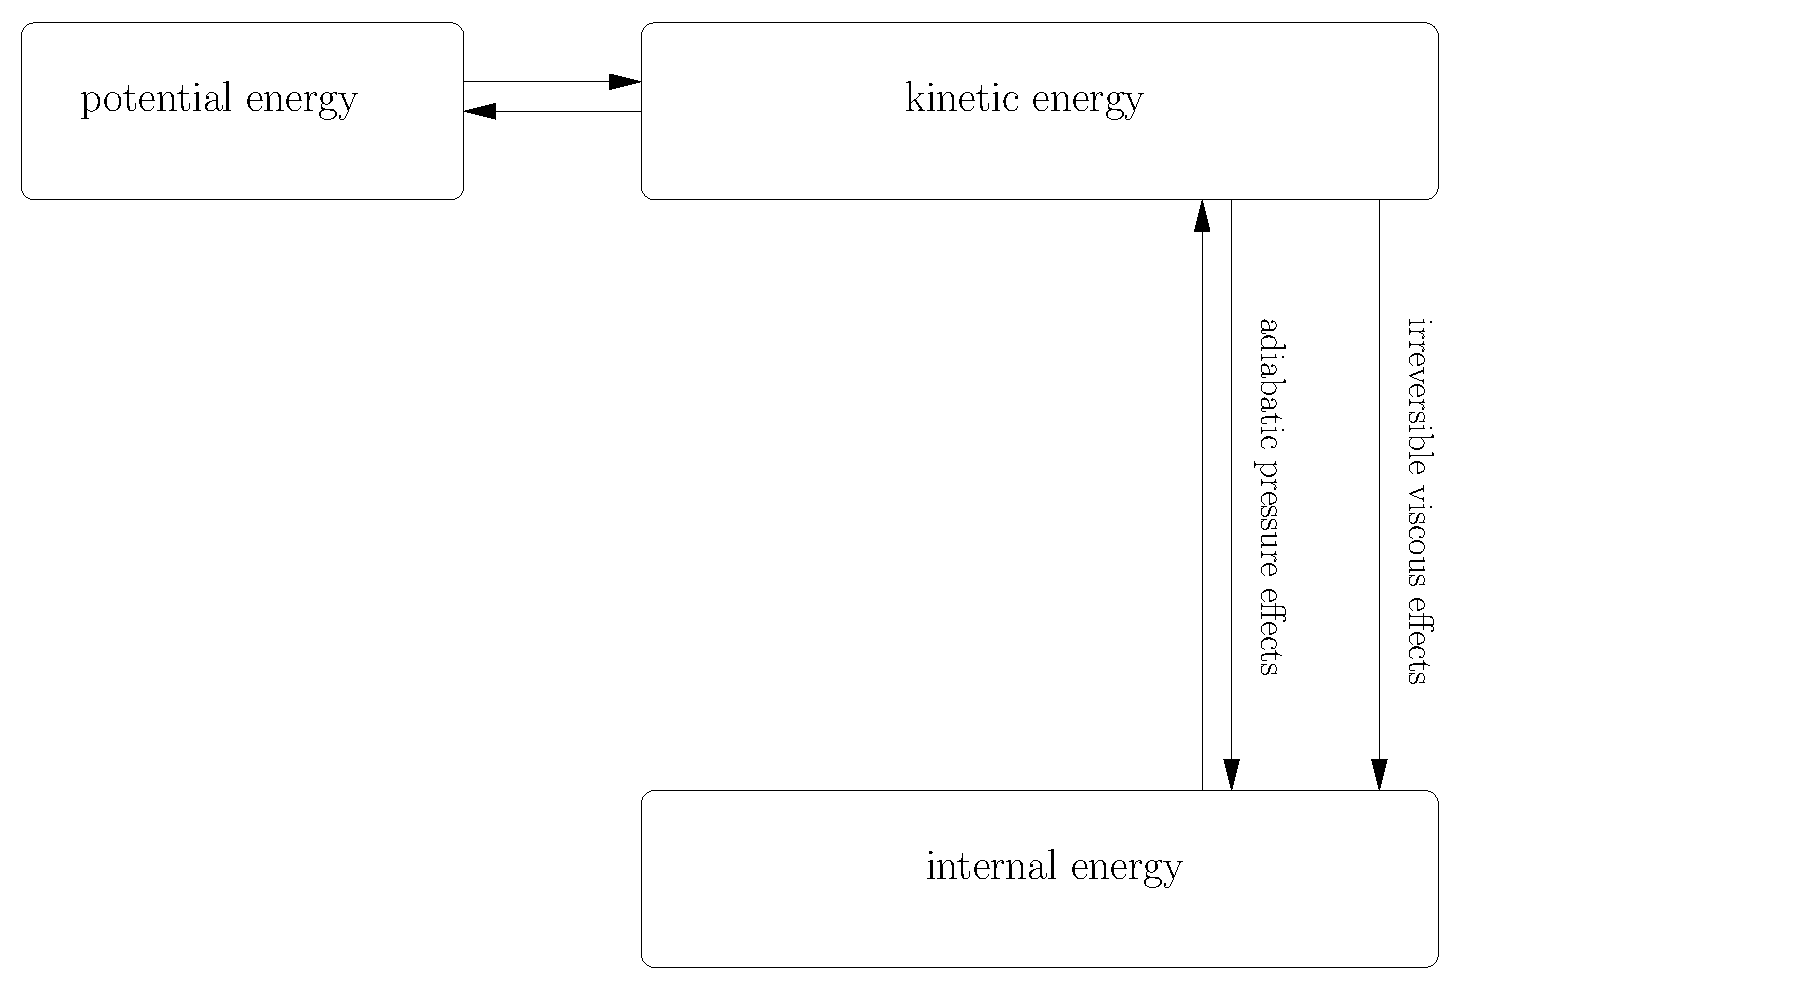
\includegraphics[width=0.7\linewidth]{chapter5/energyscheme1.eps}
\caption{Energy transfer in the unfiltered equations of fluid dynamics.} 
\label{fig:UE}
\end{figure}

One can see in figure \ref{fig:UE} the energy transfer between potential,
kinetic, and internal energy for the UE. We see that it is possible to convert
potential energy into kinetic energy and vice versa, and also kinetic energy
into internal energy and vice versa via adiabatic pressure effects. On the
other side, irreversible changes of state due to viscous effects can only lead
to an increase of internal energy and not(!) vice versa. 

\begin{figure}[tp]
\centering
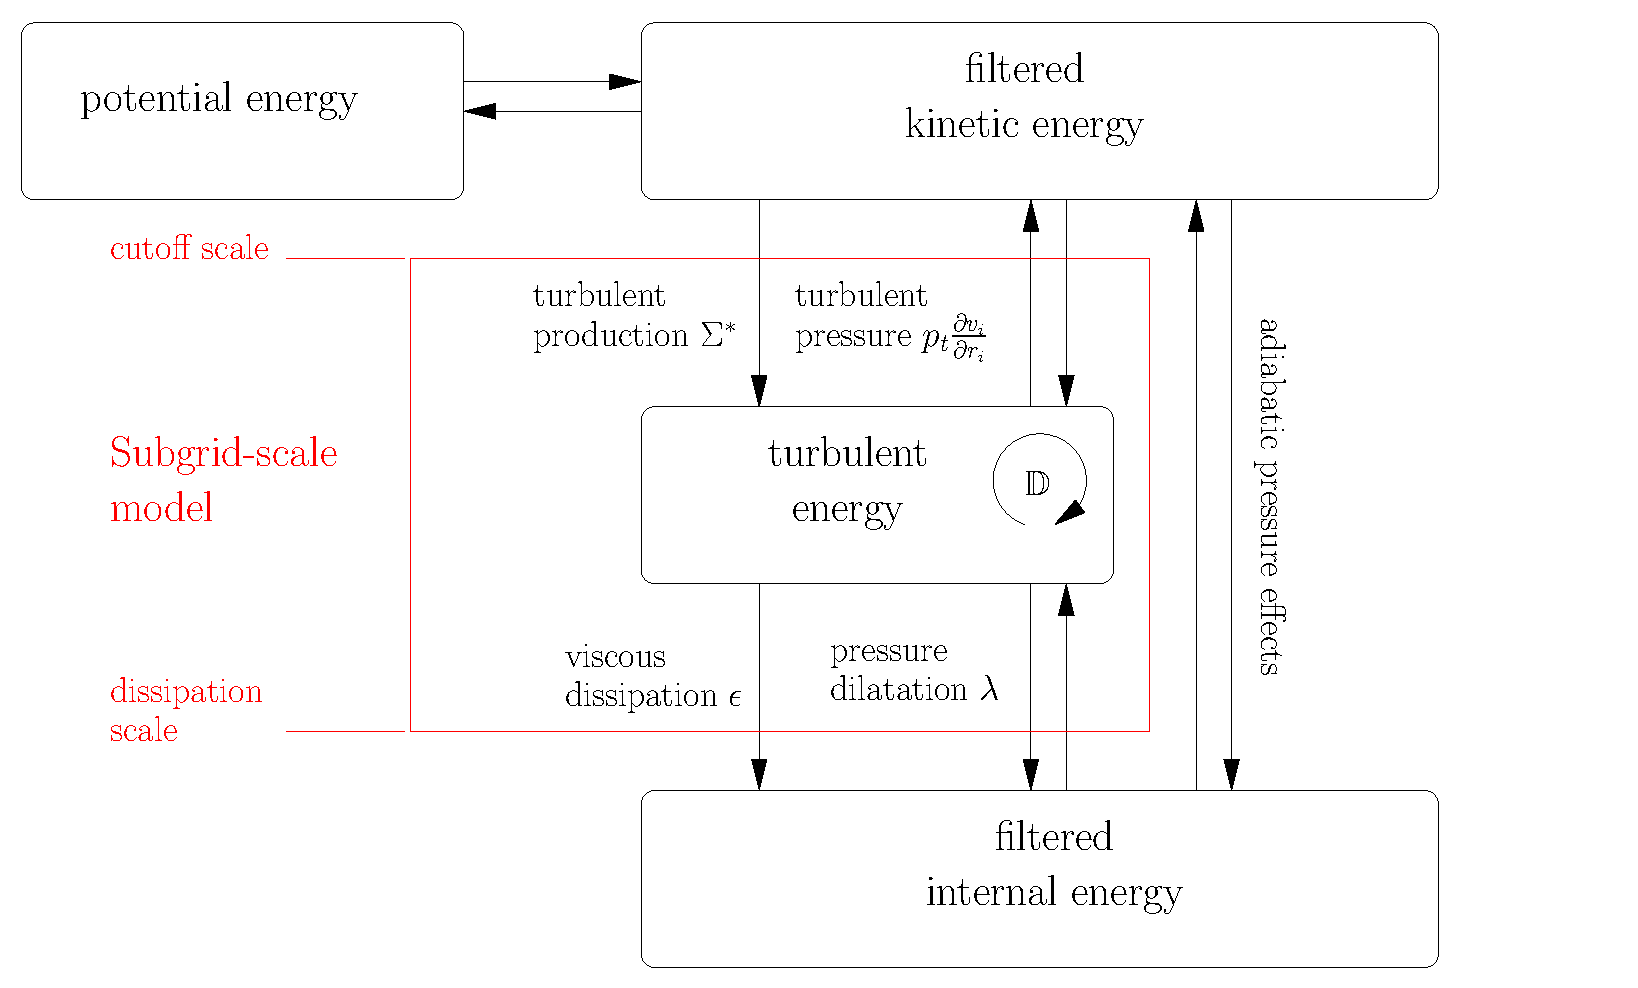
\includegraphics[width=0.7\linewidth]{chapter5/energyscheme3b.eps}
\caption{Energy transfer in the filtered equations of fluid dynamics with
Schmidt SGS.} 
\label{fig:FE}
\end{figure}

In figure \ref{fig:FE} the energy transfer for the FE with the Schmidt model is
depicted in the same schematical way. We see that the kinetic energy is now
split into two parts:
the filtered kinetic energy on resolved scales and the turbulent energy on
unresolved scales. From this picture it becomes clear that the turbulent energy
is converted to internal energy by the same processes as the filtered kinetic
energy. Also it could be converted to potential energy\footnote{Drawing the
analogy from the conversion of kinetic into internal energy one might ask if
there could be something like irreversible conversion of potential energy into
kinetic energy or perhaps vice versa. But from general relativity we know that
there is no gravity, there is only curvature of space time. It seems very
strange to imagine something like irreversible curvature of space time.}, but as
already
mentioned, this effect is neglected in the Schmidt model and therefore not
depicted here, as well as the effects due to the convective flux term. 

One very important assumption that has not yet been discussed, but is also
depicted in figure \ref{fig:FE}, is that conversion of resolved kinetic energy
into internal energy due to viscous effects is neglected. Basically all SGS
models that make use of the turbulent viscosity hypothesis, and therefore also
the Schmidt model, assume that for high Reynolds numbers the turbulent viscosity
is much greater than the real viscosity. Why this assumption can be made will
be explained in section \ref{dimanalsgs}.

The last conclusion that can be drawn from this pictures is that certain
quantities are related to the cutoff scale ($\Sigma^*,p_t$) and others are
related to the dissipation scale~($\epsilon$,$\lambda$). Nevertheless we find
that the turbulent dissipation $\epsilon$ in the Schmidt model (and also in most
other SGS models) is modeled depending on the cutoff scale $l_{\Delta}$,
although it should ultimately only depend on the dissipation scale. As we shall
see later this is a point of major concern in the development of a SGS
model for an adaptive grid code.
\subsection{Dimensional analysis}\label{dimanalsgs}
In complete analogy to the UE\footnote{See appendix \ref{dimanal}.} we can do a
dimensionless analysis for the FE with the Schmidt model. 
\subsubsection{Momentum equation}\label{dimmom}
Introducing the dimensionless quantities
\begin{align}
e_t^*= \frac{e_t}{q^2_0},\ 
p_t^*=\frac{p_t}{\rho_0 q^2_0},\ 
\tau_{ij}^{**}=\frac{\tau_{ij}}{\eta v_0/l_0}= \frac{\tau_{ij}}{\rho_0 q_0 v_0}
\end{align}
the momentum equation can be written as
\begin{align}
\frac{l_0}{t_0 v_0}\pd{t^*}\fil{\rho^*}\hat{v}^*_i
+\pd{r_j^*}\hat{v}^*_j\fil{\rho^*} \hat { v } ^*_i=&
+\frac{\rho_0 g_0 l_0}{\rho_0 v_0^2}\fil{\rho^*}\hat{g^*}_i
-\frac{p_0}{\rho_0 v_0^2}\pd{r^*_i}\fil{p^*}
-\frac{q_0^2}{v_0^2}\pd{r^*_i}p_t\\
&+\frac{\eta_0}{\rho_0 l_0 v_0 }\pd{r_j^*}\fil{\sigma^{'*}_{ij}}
-\frac{q_0}{v_0}\pd{r^*_j}\hat{\tau}^{**}_{ij}
\end{align}
From this we can estimate, that the turbulent pressure will become important,
when
\begin{align}
\frac{q_0^2}{v_0^2} \geq \frac{p_0}{\rho_0 v_0^2} \Rightarrow
\frac{q_0^2}{p_0/\rho_0} \geq 1
\end{align}
If we now introduce the turbulent Mach number 
\begin{align}
M_t=\frac{q_0}{c_s}
\end{align}
and use $\frac{p_0}{\rho_0} = \frac{c_s^2}{\gamma}$ we see that the turbulent
pressure will dominate over the thermal pressure, if
\begin{align}
M_t^2 \geq \gamma.
\end{align}

The turbulence production tensor $\hat{\tau}^*_{ij}$
becomes important compared to the stress tensor, if
\begin{align}
\rho_0 q_0 l_0 \geq \eta_0.
\end{align}
So we see that if the turbulent viscosity is greater than the physical
viscosity the turbulent production tensor will dominate over the stress tensor 
in the FE. The physical viscosity is
\begin{align}
\eta_0 \sim \rho_0 \sqrt{u_0} l_{\lambda}
\end{align}
where $u_0$ is the mean thermal energy and $l_{\lambda}$ the mean free path of
a particle, so we see that the turbulent viscosity is greater than the
physical viscosity, if
\begin{align}
\frac{q_0^2}{u_0} \geq \lra{\frac{l_{\lambda}}{l_0}}^2 \Rightarrow
\frac{q_0^2}{u_0} \geq \lra{Kn}^2,
\end{align}
which means the ratio of turbulent energy to internal energy must be greater
than the square of the Knudsen number $Kn=\frac{l_{\lambda}}{l_0}$. Since 
in any case the Knudsen number must be much smaller than one for the continuum
approximation to hold, we can practically always assume that the turbulent
production tensor will dominate over the stress tensor.\footnote{Of course this
analysis is restricted to $l_0 > l_k$, since if we resolve the fluid up to the
Kolmogorov length $l_k$ the turbulent energy will be zero. For scales smaller
than the Kolmogorov length we cannot neglect the influence of the physical 
viscosity.} This justifies our
assumption in the Schmidt model to neglect the influence of the stress tensor
completely in the momentum equation and therefore also in the kinetic energy
equation.

For completeness we also compare the gravitational force to the turbulent
pressure, which yields
\begin{align}
\frac{\rho_0 q_0^2}{\rho_0 g_0 l_0} \geq 1. 
\end{align}
Turbulence will thus dominate over gravity in the momentum equation, if the
average turbulent energy is greater than the gravitational energy. 

\subsubsection{Internal energy equation}
The internal energy equation can be analyzed in the same way as the momentum
equation using the additional dimensionless quantities
\begin{align}
e_{int}^*=\frac{e_{int}}{u_0},\ 
\lambda^* = \frac{\lambda}{\lambda_0} = \frac{\lambda}{q_0^2 v_0/l_0},\
\epsilon^* = \frac{\epsilon}{\epsilon_0} = \frac{\epsilon}{q_0^3 /l_0}.
\end{align}
This results in
\begin{align}
\begin{split}
\frac{l_0}{t_0 u_0}\pd{t^*}\fil{\rho^*} \hat{e}_{int}^*
+\pd{r_j^*}\hat{v}_j^* \fil{\rho^*}\hat{e}_{int}^* =&
-\frac{p_0}{\rho_0 v_0^2}\fil{p^*}\pd{r_j^*}\hat{v}_j^*
+\frac{\eta_0 v_0}{\rho_0 u_0 l_0}\fil{\sigma^{'*}}\pd{r_j^*}\hat{v}_j^*\\
&-\frac{q_0^2}{u_0} p_t\pd{r_j^*}\hat{v}_j^*
+\frac{q_0^2}{u_0}\fil{\rho^*}\lambda^*
+\frac{q_0^3}{v_0 u_0}\fil{\rho^*}\epsilon^*.
\end{split}
\end{align}
We see that the pressure dilatation $\lambda$ will dominate over the
pressure term if
\begin{align}
M_t^2 \geq \gamma
\end{align}
and that the turbulent dissipation $\epsilon$ will dominate over the viscous
dissipation, if 
\begin{align}
\rho_0 l_0 q_0 \lra{\frac{q_0}{v_0}}^2 \geq \eta_0 \Rightarrow
\lra{\frac{q_0}{v_0}}^2 \geq \frac{\eta_0}{\eta_t}.
\end{align}
As shown in section \ref{dimmom} $\eta_0 \ll \eta_t$, so we can always neglect
the influence of the stress tensor in the internal energy equation. This also
leads to the conclusion, that turbulence will be the only source of entropy
in the equations, since the only irreversible conversion of energy into
internal energy is via turbulent dissipation $\epsilon$.

\subsubsection{Turbulent energy equation}
For the dimensional analysis of the turbulent energy equation we need the
additional dimensionless quantity
\begin{align}
\mathbb{D}^* = \frac{\mathbb{D}}{\rho_0 q_0^3/l_0}. 
\end{align}
Inserting it together with the dimensionless quantities introduced in the
former sections yields
\begin{align}
\frac{l_0}{t_0 u_0}\pd{t^*}\fil{\rho^*}e_t^*
+\pd{r_j^*}\hat{v}_j^*\fil{\rho^*}e_t^*=&\
\frac{q_0}{v_0}\lra{\mathbb{D}^*-\fil{\rho^*}\epsilon^*}
-\frac{v_0}{q_0}\hat{\tau}^{**}_{ji}\pd{r_j^*}\hat{v_i^*}
-p_t^*\pd{r_i^*}\hat { v_i^* } - \fil{\rho^*}\lambda^*.
\end{align}
This analysis shows that the behavior of turbulent energy equation can be
completely characterized by the ratio $\frac{q_0}{v_0}$. If 
$\frac{q_0}{v_0} \gg 1$, then only diffusion $\mathbb{D}$ and dissipation
$\epsilon$ are relevant. If $\frac{q_0}{v_0} \ll 1$ then the equation is
dominated by the turbulent production term
$\Sigma^*=\hat{\tau}^{*}_{ji}\pd{r_j}\hat{v_i}$ and only if 
$\frac{q_0}{v_0} \approx 1$ do all terms contribute to the equation.

\section{Sarkar model}
The effect of compressibility on the structure of turbulence is an important
but difficult topic in turbulence modeling and is not really taken into account
by the Schmidt model. \citet{Sarkar1992} performed simulations of simple
compressible flows and investigated the influence of the mean Mach number of
the flow on the turbulent dissipation $\epsilon$ and the pressure dilatation
$\lambda$. Based on this analysis he suggested different models for these
terms, which we will describe in the following sections. These modifications
have been proven to yield good results\footnote{See \citet{Shyy1997}.} and
that's why we use them in the course of this work, when we reach the limitations
of the original Schmidt model with our simulations.
 
\subsection{Turbulent dissipation \texorpdfstring{$\epsilon$}{epsilon}}
As a major effect of compressibility from direct numerical simulation
\citet{Sarkar1992} identifies that the growth rate of kinetic energy decreases
when the initial turbulent Mach number increases. This means that the
dissipation of kinetic energy (and therefore also for the turbulent
energy) increases with the turbulent Mach number $M_t$ and
\citet{Sarkar1992} suggests accounting for this effect by using
\begin{align}
\epsilon=C_{\epsilon}\frac{q^3}{l_{\Delta}}(1+\alpha_1 M_t^2)
\end{align}
with $\alpha_1=0.5$ as a model for the dissipation of turbulent energy.

\subsection{Pressure dilatation \texorpdfstring{$\lambda$}{lambda}}
Based on a decomposition of all variables of the equation for instantaneous
pressure\footnote{For a derivation see appendix \ref{diveq}.} 
\begin{align}
\pdd{r_i} p = \pdd{t}\rho- 
\frac{\partial^2}{\partial r_i \partial r_j}(\rho v_i
v_j-\sigma'_{ij})\label{eq:instpres}
\end{align}
into a mean and a fluctuating part and comparisons with direct numerical
simulations of simple compressible flows \citet{Sarkar1992} proposed a different
model for the pressure dilatation 
\begin{align}
\lambda=\alpha_2 M_t \hat{\tau}^*_{ij} \ppd{r_j}{\hat{v}_i} 
- \alpha_3 M_t^2 C_{\epsilon}\frac{q^3}{l_{\Delta}}
- 8 \alpha_4 M_t^2 p_t \ppd{r_k}{\hat{v}_k}
\end{align}
with $\alpha_2=0.15$,$\alpha_3=0.2$ obtained from a curve fit of the model with
DNS simulation. Unfortunately \citet{Sarkar1992} does not specify a value for
$\alpha_4$, so there is some confusion in the literature about it. For example
\citet{Shyy1997} set $\alpha_4 = 0$ and still found the Sarkar model in good
agreement with their DNS simulation. In this work, we adopt a value of 
$\alpha_4 = \alpha_2^2/2$, which was suggested in a work by
\citet{Schmidt2007a}.

